\documentclass{bioinfo}
\usepackage{multirow}
\usepackage{xr}
\usepackage[export]{adjustbox}
\usepackage{float}
\usepackage[caption = false]{subfig}
\usepackage{graphicx}

\copyrightyear{2015} \pubyear{2015}

\access{Advance Access Publication Date: Day Month Year}
\appnotes{Manuscript Category}

\externaldocument{supplement}

\begin{document}
\firstpage{1}

\subtitle{Subject Section}

%\title[Pipe]{Pipe: Pipeline for detecting viral integration from Next Generation Sequencing data}
\title[ViFi]{ViFi: Viral integration and mRNA fusion identification}
\author[Nguyen \textit{et~al}.]{Nam-phuong Nguyen\,$^{\text{\sfb 1}}$, Viraj Deshpande, 
Jens Luebeck\,$^{\text{\sfb 1}}$ and Vineet Bafna\,$^{\text{\sfb 1,*}}$}
\address{$^{\text{\sf 1}}$Computer Science and Engineering, University of California, San Diego, La Jolla, 92093, USA.}

\corresp{$^\ast$To whom correspondence should be addressed.}

\history{Received on XXXXX; revised on XXXXX; accepted on XXXXX}

\editor{Associate Editor: XXXXXXX}

\abstract{\textbf{Motivation:}  An estimated 12\% of all human cancers are caused by oncoviruses (i.e., a virus linked to cancer), with more than 80\% of the cases occurring in developing nations.  In cancers such as cervical cancer and hepatocellular carcinoma, the integration of the viral genome into the host cell's genome is an important factor tumor genesis.  The standard approaches to viral integration detection identify paired end reads that map to both the human and viral references.  However, read-based reference mapping can have difficulty identifying integration sites from fast evolving viruses or from novel viruses.\\
\textbf{Results:} We present ViFi, a viral integration detection tool that uses both reference-based read mapping and a phylogenetic-based approach to identify viral reads.  Key to this framework is the use of profile Hidden Markov models used to represent the viral family of interest, allowing the detecting of highly mutated or novel viral sequences belonging to that family.  In addition, ViFi use mappability scores to reduce false positive detections.  ViFi can be run on both WGS and RNA-seq data, allowing for both the detection of integration sites and fusion transcripts.  We compare Viral-HMM to VERSE and VirusFusionSeq on both simulated NGS data and real biological data with experimentally verified integration sites.  Our results show that ViFi is more sensitive in detecting integration sites, while also having a lower false positive detection rate.\\
\textbf{Availability:} ViFi is availble on github at ...\\
\textbf{Contact:} \href{ndn006@eng.ucsd.edu}{ndn006@eng.ucsd.edu}\\
\textbf{Supplementary information:} Supplementary data are available at \textit{Bioinformatics}
online.}

\maketitle

\section{Introduction}
Viral infection and integration plays key roles in tumorigenesis, however, determining the causative factors has been challenging.  Difficulties include the long latency period between infection and cancer formation (between 15 to 40 years for some cancers), the viruses that cause cancer in some patients often do not cause cancer in many other patients, and some viruses are indirect carcinogens (i.e., viral genes are not present in the tumor cells)~\cite{Hausen2009}.  Additional difficulties in understanding viral-related cancers is that the human cancer viruses span a wide range of virology, including retroviruses, positive-stranded RNA viruses, and small and large DNA viruses.  While these groups of viruses have different cellular targets and different methods for proliferation, one key insight is that some of these viruses (Human papillomavirus (HPV), Molluscum contagiosum virus (MCV), Hepatitis B virus (HBV), and Human T-lymphotropic virus (HTLV)) have mechanisms for integrating directly into the host genome, and these viruses are clonal within individual tumors cells, suggesting that integration may lead to cellular proliferation and cancer formation~\cite{Moore2010}.

Identifying integration points is vital to understanding viral-related tumorgenesis.  Studies of the impact of viral integration on tumorgenesis have found evidence of recurrent genomic hotspots in both HBV-related hepatocellular carcinoma (HCC; ~\cite{Ding2012, Khoury2013}) and HPV-related cervical cancers~\cite{Schmitz2012}.  In these studies recurrent integrations were often found in or near known oncogenes such as TERT, MYC, and MLL4, suggesting that integration occurs randomly across the genomic, however over the course of tumor formation progression, integrations in key genomic regions may provide a selective advantage for the host cells, resulting in recurrent integrations across different samples.  

The majority of HPV and HCC tumors, however, do not contain recurrent integrations.  Thus, focusing on just recurrent integrations may result in an incomplete story on the role of viral integration on tumor formation.  Integration can result in altered mRNA expression of flanking regions and viral-human fusion mRNA transcripts~\cite{Tang2013}.  Viral-human fusion transcripts can alter functional pathways, as in the case of the viral-human fusion transcript HBx-LINE1~\cite{Lau2014}, which acts as a sponge for miRNA-122 and promoted hepatic cell epithelial-mesenchymal transition (EMT)-like changes and increased susceptibility to induced tumor formation~\cite{Liang2016}.  

Traditionally, viral integration was detected using PCR-based methods, however due to the labor intensive process of running the PCR experiments, and the low coverage and depth of PCR techniques, integration events were difficult to identify.  With the advent of Next Generation Sequencing (NGS) technology, human genomes can now be sequenced with high coverage and high sequencing depth thus making it more feasible to accurately identify the location of the viral integrations within the human host genome.  Indeed, many pipelines have recently been developed for the detection of viral integration from paired end Illumina data (VirusSeq~\cite{Chen2013}, VirusFinder~\cite{Wang2013}, VirusSeqFusion~\cite{Li2013} in 2013; VERSE~\cite{Wang2015}, Virus-Clip~\cite{Ho2015}, and Vy-PER~\cite{Forster2015} in 2015).  While each pipeline varies in how detection is performed, the overarching theme is similar: identify single end or paired end reads that map to both the human and viral reference genome.  Paired end reads in which one read maps to a viral reference and the other read maps to a human reference (known as \emph{chimeric paired end reads}) are indicative of a potential integration event.  Single end reads that partially map to a human reference and viral reference are known as \emph{split end reads} and are useful for determining the exact integration point in the human chromosome.  The key step for these methods is the use of a reference-based read mapper (i.e., BLAST~\cite{Altschul1990}, BLAT~\cite{Kent2002}, BowTie2~\cite{Langmead2012}, or BWA~\cite{Li2009}) to categorize the read pairs.  These methods perform pairwise sequence alignment between the query sequence and a reference sequence in order to determine if a) the query sequence is related to the reference, and b) what is the optimal alignment of the query sequence to the reference sequence.

Detecting viral integrations from NGS technology is still challenging.  For example, the integrations from ~\cite{Hu2015} have been challenged as false positives integrations as a result of PCR sequencing artifacts~\cite{Dyer2015}.  Indeed, one of the large problems with viral integration methods is separating out true integrations from false positives integrations, which can result from shared repeat regions between human and viral genomes~\cite{Forster2015}.  

One of the shortcomings of reference-based pairwise alignment approaches for performing read alignment is the difficulty in aligning reads from novel or evolutionarily divergent organisms~\cite{Brenner1998,Park1998}.  This can result in a poor alignment between the query sequence and the closest reference sequence or can even result in the failure to detect any evolutionary relationship between the query sequence and the known reference sequences.  An alternative approach is to first represent the relationships between the reference sequences using an evolutionary model.  Then a given query sequence can be scored against the model, and if the score is significant, fitted to the model.  One example of a commonly used evolutionary model is a \emph{profile Hidden Markov Model} (HMMs;~\cite{Eddy1998}). HMMs are a statistical model for representing an MSA, and HMMs have been used to detect membership of query sequences to protein families~\cite{Finn2010}, align fragmentary sequences~\cite{Eddy1998}, and identify viral fragments from metagenomic samples~\cite{Skewes-Cox2014}.  Given a query sequence, the profile HMM can produce scores that represent the probability of the model generating the sequence, as well as the best alignment of the query sequence to the model.

Previous research has shown that profile HMMs can have difficulty in recognizing sequences that come from evolutionarily divergent families, and that using an ensemble of profile HMMs (eHMMs)~\cite{Mirarab2012,Nguyen2014,Nguyen2015,Nguyen2016_hippi} can improve recognition rates.  The eHMMs technique has been shown to have better detection and alignment of query sequences to a given model compared to the single HMM approach, and as a result, better downstream downstream phylogenetic analyses. 

\section{Our approach}
We present \textbf{V}irus \textbf{I}ntegration and \textbf{F}usion \textbf{I}dentification (ViFi), a new pipeline for detection of integration sites (Fig.~\ref{flowchart}).  Unlike other integration detection pipelines that use reference-based alignment mapping for identifying viral reads, ViFi uses a combination of reference-based alignment mapping and ensemble of profile HMMs to identify viral reads.  

\paragraph{\textbf{Pre-processing.}} ViFi begins with a pre-processing step (see Fig.~\ref{flowchart}a) that builds an BWA index on the human reference genome and viral genomes (Hg19+viral index).  In addition, ViFi takes the genomes from the viral family and estimates a multiple sequence alignment (MSA) on each family using PASTA~\cite{Mirarab2014}.  A maximum likelihoood (ML) tree is estimated from the alignment using RAxML~\cite{Stamatakis2014}.  Next, ViFi builds an ensemble of HMMs from the alignment and tree using HIPPI~\cite{Nguyen2016_hippi}.  Briefly, a profile HMM is computed on the input MSA.  Next, the ML tree is partitioned into two subtrees by taking its centroid edge (i.e., the edge that best separates the tree into two subtrees with roughly equal number of leaves).  Profile HMMs are then built on the alignments induced by the leaf set of each of the subtrees.  This process repeats recursively on each subtree until there is at most 10 sequences in the subtree.  This results in a collection of nested hierarchical profile HMMs which we call the ensemble of HMMs.  This pre-processing step of building the ensemble of HMMs only needs to be run once for each viral family of interest.

\paragraph{\textbf{Identification of candidate reads.}} Similar to other existing viral integration detection pipelines, the first step of ViFi is to align each paired end read to the Hg19+viral index.  The paired end reads are separated into four different groups: i) reads in which both paired end reads mapped Hg19 or both to the viral genomes, ii) paired end reads in which one end mapped to Hg19 and the other to a viral genome, iii) paired end reads in which one end mapped to Hg19 and the other is unmapped, and iv) all other reads.  Typically, most existing viral integration detection pipelines focus on the set of reads in group ii) and discard reads found in group iii).  However, a read that is viral in origin might be unmapped because it is too evolutionarily divergent from the set of known viral genomes.  Our method attempts to rescue paired end reads in this category by scoring the unmapped reads against the ensemble of HMMs created in the pre-processing step.  If a read has a sufficient score to one of the HMMs in the ensemble (E-value of 0.01 or lower), then the read is marked as a viral read and the paired end read is put into the candidate set, along with all reads from group ii).  This step allows the detection of novel or evolutionarily divergent viral sequences belonging to the same family.  The last step is to infer integration from the set of candidate reads.  

\paragraph{\textbf{Identification of integration point.}}  The set of candidate reads are ordered by coordinates of the human genomic position.  Read pairs with poor mappability scores, defined as Duke Uniqueness Score~\cite{unknown} less than 0.33 or MAPQ score less than 10 are removed.  These removed reads represent reads that might map to multiple locations.  The remaining read pairs within 300 bps of each other are clustered into a group of read pairs supporting the integration point.  The reads remaining in the cluster are then considered highly supported reads (i.e., have high mapping score).  

%Any paired end reads in which one or more ends did not map to the reference are put into a candidate set.  From the candidate set, all reads are scored against the ensemble of HMMs, and those that score above a threshold are marked as viral.  paired end reads that have at least one read mapping to the human reference and one marked viral are considered candidate integration points.  Integration points with at least three paired end reads supporting the integration are listed as positive integrations.


%paired end reads in which at least one end did not map to the human reference are put into a candidate set.  All reads in the candidate set are scored against each HMM in the ensemble using nhmmer from the HMMER suite of tools~\cite{Eddy1998}.  Any read that scores above a threshold $T$ is marked as viral.  paired end reads in which at least one end maps to the human reference and at least one end is marked as viral are considered as candidate integration event.  Any read that maps to the human reference and is marked as viral is candidate split read and is used to identify the integration point on the human genome.  If an integration point is covered by a split read, we can identify the exact integration location on the human genome.  However, as not all integration events are covered by split reads, we also identity integration points with a range (ADD MORE DETAIL) defined by the insert size.  Integration points that are supported by three or more paired end reads are outputted as  true integration points.

\begin{figure*}[htpb]
  \centering
  \subfloat[Pre-processing]{\includegraphics[width=4in,frame]{{preprocess}.pdf}}\\
  \subfloat[Pipeline]{\includegraphics[width= 4in,frame]{{mapping}.pdf}}
\caption[Overview of integration detection pipeline.]
{\label{flowchart}  {\bf Overview of integration detection pipeline.}  Integration detection is split into two phases.  In the a) pre-processing step, a BWA index is created from the human reference genome and input viral genomes (Hg19+viral).  In addition, a multiple sequence alignment (MSA) is estimated from the viral genomes, and an maximum likelihood (ML) tree is estimated from the alignment.  The MSA is decomposed into an ensemble of profile Hidden Markov models.  In the b) viral detection step, the paired end reads are mapped against the Hg19+viral index.  Candidate paired end reads are selected if, i) one end of the read maps to the human genome and the other end maps to a viral genome, or ii) one end of the read maps to the human genome and the other end scores high against the HMM ensemble.  All other reads are discarded.  The integration point is then inferred from the set of candidate reads.
% i) reads in which both paired end reads mapped Hg19 or both to the viral genomes, ii) paired end reads in which one end mapped to Hg19 and the other to the viral genomes, iii) 
%Any paired end reads in which one or more ends did not map to the reference are put into a candidate set.  From the candidate set, all reads are scored against the ensemble of HMMs, and those that score above a threshold are marked as viral.  paired end reads that have at least one read mapping to the human reference and one marked viral are considered candidate integration points.  Integration points with at least three paired end reads supporting the integration are listed as positive integrations.
}
\end{figure*}


\begin{figure}[htpb]
  \centering
  \includegraphics[width=0.6\linewidth]{{ehmm}.pdf}\\
\caption[Ensemble of HMMs technique.]
{\label{ehmm}  {\bf Algorithm for generating the ensemble of HMMs.}  The input is a initial MSA and a maximum likelihood (ML) tree that has been estimated for the MSA. The algorithm begins by adding the HMM built on the MSA to the ensemble. If the MSA has more than 10 sequences, the ML tree is decomposed into two subtrees by deleting the centroid edge (i.e., the edge that produces a maximally balanced split of the sequence set into two sets). The subtrees are used to generate induced alignments. HMMs are built for each induced alignment and added to the ensemble. The process iterates on those subtrees that meet the criterion for decomposition (subset size more than max(10, n/10), where n is the number of sequences in the initial MSA, and mean pairwise sequence identity less than 0.4).}
\end{figure}

% (see Fig.~\ref{viral_discovery}).  The basic idea is to first map all paired end reads to both a human reference genome and to known viral reference genomes.  Second, paired end reads in which both reads map to the human reference are removed.  Third, paired end reads in which both reads map to viral genomes are used to identify potential viral candidates.  Fourth, for read pairs in which one read maps to a viral reference and the other read maps to a human reference (known as \emph{chimeric reads}) are indicative of a potential integration event.  Finally, in some cases, a single read might partially map to a human reference on one end and to the viral reference on another end.  These reads are known as \emph{split-end reads} and are useful for determining the exact integration point in the human chromosome.  The key step for these methods is the use of a reference-based read mapper (i.e., BLAST~\cite{Altschul1990}, BLAT~\cite{Kent2002}, BowTie2~\cite{Langmead2012}, or BWA~\cite{Li2009}) to categorize the read pairs.  These methods perform pairwise sequence alignment between the query sequence and a reference sequence in order to determine if a) the query sequence is related to the reference, and b) what is the optimal alignment of the query sequence to the reference sequence.
%For example, a recent study found recurrent HPV integrations in several oncogenes~\cite{Hu2015}.  The authors hypothesized that HPV might first integrate randomly across the genome, however over the long term, integrations at key loci may provide a selective advantage to the host cells, resulting in hot-spots genes with recurrent integration.  Another HPV study found that more than half of HPV-infected tumors had viral-human fusion transcripts, suggesting that the host-spot locations are transcriptionally active~\cite{Schmitz2012}.  In many cases, integrated HPV genomes have a disrupted E2 gene; the suppression of the viral E2 gene can result in suppression of the tumor suppressor p53 gene in humans~\cite{Akagi2014}. Another recent study found that copy number variations (CNV) were significantly increased near HBV integration locations which the authors suggest that integration may cause chromosomal instability~\cite{Sung2012}.  In addition, the authors found recurrent integration in or near several oncogenes, including TERT, which produces an enzyme that is found in high activity in cancer cells.  Thus, being able to identify integration locations can help us detect hotspot genes with recurrent integrations, identify fusion transcript, find oncoproducts, and examine the chromosomal stability around the integration point.  All of these factors can help us better understand the mechanisms of how a normal cell might transform into a tumor cell upon infection.


%\begin{figure}[htpb]
%  \centering
%  \includegraphics[width=1\linewidth]{{viral_discovery_1}.pdf}\\
%\caption[paired end sequencing viral integration discovery pipeline.]
%{\label{viral_discovery}  {\bf Viral integration and discovery.}  1) The human genome (represented in blue) has a viral integration event (represented in red).  2) The DNA is extracted and fragmented.  Some fragments will consist of only human DNA, some fragments will consist of viral DNA, and some fragments will be chimeric.  3) The fragments are sequenced via Illumina paired end sequencing technology and mapped to onto a human reference and a viral reference.  3) Depending on which reference(s) the paired end reads map onto, pairs are grouped into four categories: a) human, b) viral, c) chimeric, or d) split.}
%\end{figure}

\section{Methods}
We compare ViFi with VERSE~\cite{Wang2015} and ViralFusionSeq~\cite{Li2013} on both simulated and real biological datasets.  We selected VERSE and ViralFusionSeq for comparison as VERSE is among the most recent viral integration tools and has been shown to outperform VirusFinder and VirusSeq, and ViralFusionSeq is the only viral integration tool available on NIH HPC system.  We report the true positive and false positive integration points reported on the simulated datasets, and the true positive integration points reported on biological datasets with experimentally verified integration points.  Finally, we report the number of fusion transcripts detected from the matched RNA-seq datasets, and the number of those transcripts that are supported from the matched WGS datasets.

\subsection{Datasets}
We benchmarked the different methods on both simulated and on real biological datasets, including two biological datasets with experimentally verified integration points.  The biological datasets included both WGS and RNA-seq datasets. These datasets include simulated WGS of genomes containing integrated HPV, WGS from HCC samples taken from patients with HBV~\cite{Sung2012}, RNA-seq datasets from HCC cell lines infected with HBV~\cite{Lau2014}, matched WGS data from normal and tumor cervical samples taken from the The Cancer Genome Atlas (TCGA).  Details for each of the datasets is provided below, and a summary is provided in Table~\ref{table:data}.

\subsubsection{HPV simulated WGS datasets (HPV-Sim)}
We simulated 16 human genomes with HPV integrations.  In order to examine the impact of viral sequence divergence on integration detection, we simulated different strains of HPV by evolving HPV16 down a phylogenetic tree with differing branch lengths.  We grouped the simulations into three categories, depending on the integrating virus strain's similarity to the reference HPV16 strain: easy (99\% similarity), medium (95\% similarity), and hard (90\% similarity).  In addition, we generated one additional dataset with Alouatta guariba papillomavirus 1 (AgPV1), a papillomavirus genome not included in the set of viral reference genomes to simulate detection of a novel HPV virus.  AgPV1 is 44\% similar to HPV16 and is 65\% similar to the most closely related sequence in the set of reference genomes.


\subsubsection{HCC Sung 2012 WGS dataset (HCC-WGS)}
88 HCC samples (81 HBV-positive and 7 HBV-negative; both tumor and adjacent tissue) were sequenced by Sung et al.~\cite{Sung2012}.  The authors identified recurrent breakpoints (4 or more samples) in known oncogenes/oncogeneic regions (FN1, TERT, MLL4, CCNE1, ROCK1, SENP5).  A total of 399 breakpoints were identified across the 88 samples.  To confirm recurrent breakpoints, the authors randomly selected 32 breakpoints in six affected genes from 21 samples and validated 22 of these (72\%) via PCR.  Our study used the same 21 samples in our comparison.

\subsubsection{HCC Lau 2014 cell line RNA-seq dataset (HCC-RNAseq)}
Whole transcriptomes from four HCC cell lines were analyzed using RNA-seq~\cite{Lau2014}.  11 chimeric HBV-human fusion transcripts in three of the cell lines were detected and validated using Sanger sequencing.  Our study used the original six cell line sequencing data.  

\subsubsection{TCGA Cervical cancer datasets (TCGA-CESC)}
We found 68  patient cervical tumor samples in the TCGA database~\cite{TODO} with matched WGS and RNA-seq tumor sequencing data.  Of the 68 samples, 28 samples overlapped with the Tang et al. study~\cite{Tang2013} which examined the landscape of mRNA viral fusion events across the TCGA dataset.  


\begin{table*}[htb]
\centering
\caption{\textbf{Overview of datasets}.  We provide an overview of the datasets used throughout this study.  }
\label{table:data}
\begin{tabular}{|l|l|l|r|r|}
\hline
Dataset name & Type & Simulated/Biology & Number of samples & Source \\ \hline
HPV-Sim & WGS &Simulated& 16 & Generated for this study \\ \hline
HCC-WGS & WGS & Experimental&20 & ~\cite{Sung2012} \\ \hline
HCC-RNAseq & RNA-seq & Experimental&6 & ~\cite{Lau2014} \\ \hline
TCGA-CESC & WGS and RNA-seq &Experimental& 69 & TCGA~\cite{TODO} \\ \hline 
\end{tabular}
\end{table*}
\section{Results}

\subsection{HPV-Sim Simulated Datasets}
We ran all three methods, including ViFi both with and without the HMMs, on the simulated datasets that contained 25 viral integrations per dataset (Fig.~\ref{sim_results}).  All methods were run on a dedicated compute node with 24 CPUs and given 48 hours to complete.  Only ViFi and VERSE completed within the allotted time; ViralFusionSeq failed to complete on any of the datasets.  ViFi required an average wall clock running time of 7 hours and 30 minutes (minimum of hours 13 minutes to maximum of 8 hours and 2 minutes); VERSE required an average of 8 hours and 19 minutes to complete per dataset (minimum of 6 hours and 1 minute to a maximum of 9 hours and 19 minutes).  

Both ViFi (both with and without HMMs) and VERSE have high precision and recall on the easier datasets (95-99\% similarity with HPV16).  However, when the integrated virus has only 90\% similarity to HPV16, VERSE's precision and recall drops by one half.  ViFi, on the other hand, is still able to accurately detect the highly mutated simulated HPV16 sequence.  On the dataset that contains the novel AgPV1 sequence, only ViFi with the HMMs is able to accurately detect integration events (88\% recall and 93\% precision).  ViFi without the HMMs is only able to detect 20\% of the integrations, but with high precision.  VERSE is unable to detect any integration events.  

Interestingly, VERSE takes significantly longer when it can detect more integrations.  When no integrations are detected, it takes roughly 6 hours to complete, however, this time jumps by two to three hours when it detects 20 or more integrations.  This made VERSE impossible to complete on any of the datasets with 1000 integrations.  ViFi, on the other hand, had an average increase of running time of 32 minutes when increasing the number of simulated viral integrations from 25 to 1000 integrations, without any loss of recall or precision (Fig. S1).


\begin{figure}[htpb]
  \centering
  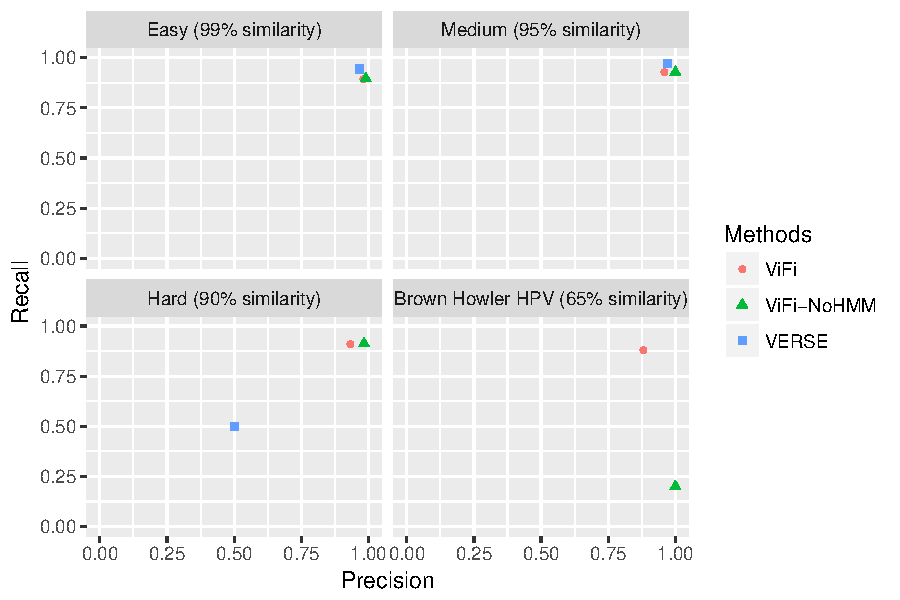
\includegraphics[width=1\linewidth]{{results/simulation.main}.pdf}\\
\caption[Precision-recall on simulated datasets.]
{\label{sim_results}  {\bf Precision-recall on simulated datasets.}  We report the recall and precision for four different model conditions.  We show results for when we include the usage of the  ensemble of HMMs in detecting viral reads (Default) and when we exclude the usage of the ensemble of HMMs (Default-NoHMMs).  The first three model conditions (easy, medium, and hard) vary the percent similarity of simulated HPV16 genomes to the reference HPV16 genome, with five replicates per simulation.  The last model condition uses Alouatta guariba papillomavirus 1 (AgPV1), an HPV genome not included in the set of viral genomes to simulate detection of a novel HPV virus.  AgPV1 is 44\% similar to HPV16.  There are 25 simulated integrations per dataset.  VERSE failed to detect any viruses on the AgPV1 model condition.  All datasets were simulated with 25x coverage.}
\end{figure}


\subsection{HCC-WGS and HCC-RNAseq datasets}
Of the 21 experimentally verified integration points in the HCC-WGS dataset, ViFi was able to detect 17 of the integration points, and VERSE was able to detect 16.  In the HCC-RNAseq datasets, both ViFi and VERSE both recovered 10 out of 11 verified fusion mRNA points.

\begin{figure}[htpb]
  \centering
  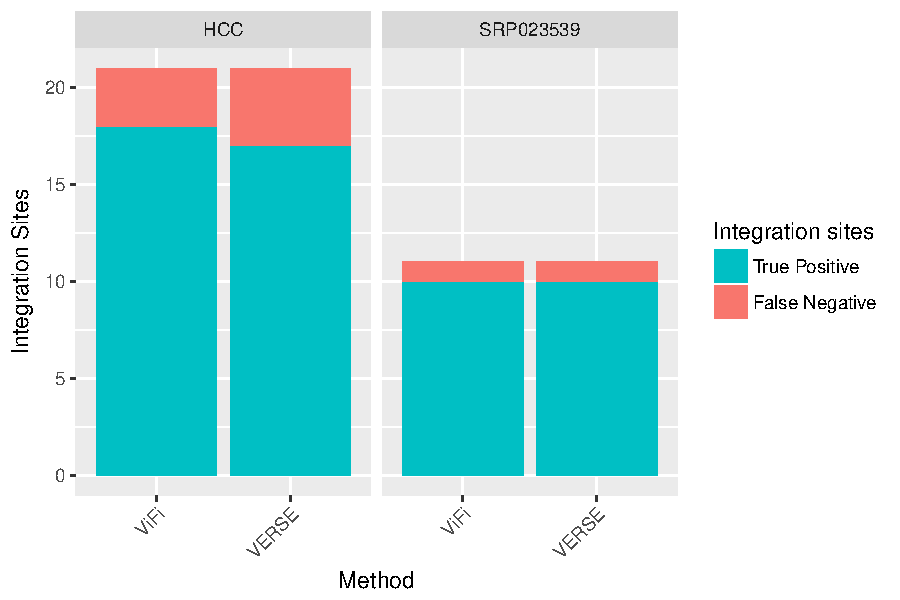
\includegraphics[width=1\linewidth]{results/hcc.pdf}\\
\caption[Recovery of experimentally verified integration sites from biological datasets.]
{\label{bio_results}  {\bf Recovery of experimentally verified integration sites.}  We report the number of experimentally verified integration sites recovered from biological datasets for our method and VERSE.  The datasets include the HCC WGS dataset from the Sung et al. 2012 study (21 experimentally validated integration sites) and the HCC RNAseq cell line dataset from the Lau et al. 2014 study (11 experimentally validated integration sites).}
\end{figure}


\subsection{TCGA-CESC comparison study}
We compared fusion mRNA events detected by ViFi and VERSE to the results reported in the Tang et al. study~\cite{Tang2013} on 28 TCGA-CESC samples.  For each sample, we ran ViFi on the WGS data to detect viral integrations.  For each viral integration reported by ViFi, we report whether or not each of the three methods also found one or more fusion mRNA events within a 100kb interval around that integration point.  In any case in which VERSE or the Tang study found a fusion mRNA event, ViFi also found that event (Fig.~\ref{venn_diagram}).  In addition, ViFi found five fusion mRNA events that was also supported supported by the WGS data that neither VERSE or the Tang study identified.  Closer inspection of these events show strong evidence that these fusion mRNA sequences are real events that were missed by VERSE and the original Tang et al. 2013 study (Fig. S2).

\begin{figure}[htpb]
  \centering
  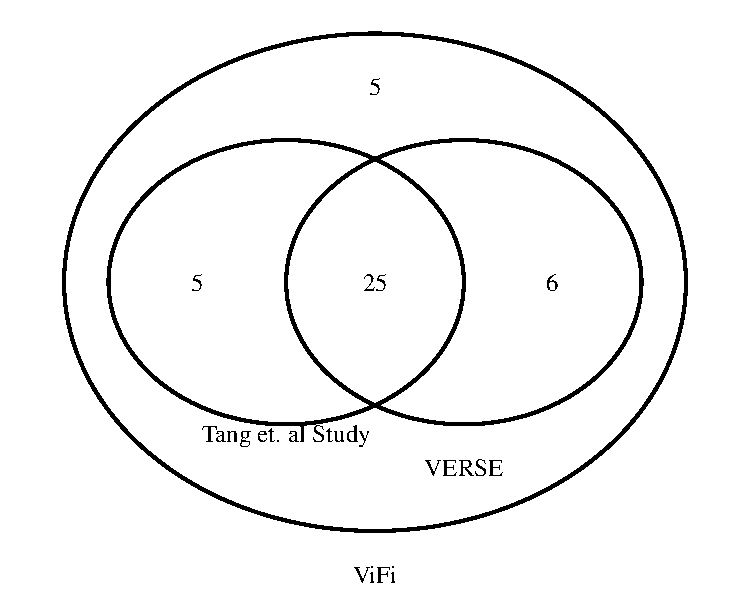
\includegraphics[width=1\linewidth]{results/tcga_triple.pdf}\\
\caption[Venn diagram of fusion reads recovered from the RNAseq data from Larsson 2013 study]
{\label{venn_diagram}  {\bf Venn diagram of fusion read integration points recovered from the TCGA-CESC samples with matched RNA-Seq and WGS sequencing.}  We show a Venn diagram of the overlap of the WGS integration points with a matching mRNA event within 100kb reported by ViFi, VERSE, and the Tang et al. 2013 study on the TCGA-CESC samples with both RNA-Seq and WGS sequencing matched pair data.  }
\end{figure}

\subsection{TCGA-CESC results}
We applied ViFi to 68 cervical cancer samples with matched WGS and RNA-seq data.  We found integrations in 51 samples (226 integrations total), of which 49 contained fusion mRNA sequences (392 fusion mRNA sequences total).  While a few of the fusion mRNA breakpoints were found within close proximity of the genomic integration breakpoint (27\% were within 100 bps), the majority were more than 1000 bps away (66\%).  This suggests that the majority of the fusion reads have undergone some splicing event.

\begin{figure}[htpb]
  \centering
  \includegraphics[width=1\linewidth]{results/{wgs.rna.histogram.distances}.pdf}\\
\caption[Distance of fusion mRNA breakpoint to nearest WGS integration breakpoint.]
{\label{distance_breakpoint}  {\bf Histogram of distance of fusion mRNA breakpoint to nearest WGS integration breakpoint.}  }
\end{figure}

We applied ViFi to 68 cervical cancer samples with matched WGS and RNA-Seq data.  We found integrations in 51 samples, of which 49 contained fusion mRNA sequences.  Importantly, genomic segments with integrations had increased expression of nearby human mRNA (2.5 fold increase), with significantly higher expression when human-viral fusion mRNA are present (5.5 fold increase).  Surprisingly, we found that integration also results in the expression of proximal LTR and LINE elements (3.5 to 5.3 fold increased expression when fusion mRNA is present).   Guided by previous results that implicate fusion HBV-LINE1 with increased tumor susceptibility in HCC (Lau et al. Cancer Cell 2014), our findings highlight the need to explore the roles of LINE and LTR elements in HPV pathogenesis in cervical cancer.  suggest a novel mechanism of HPV pathogenesis in cervical cancer.


\begin{figure}[htpb]
  \centering
  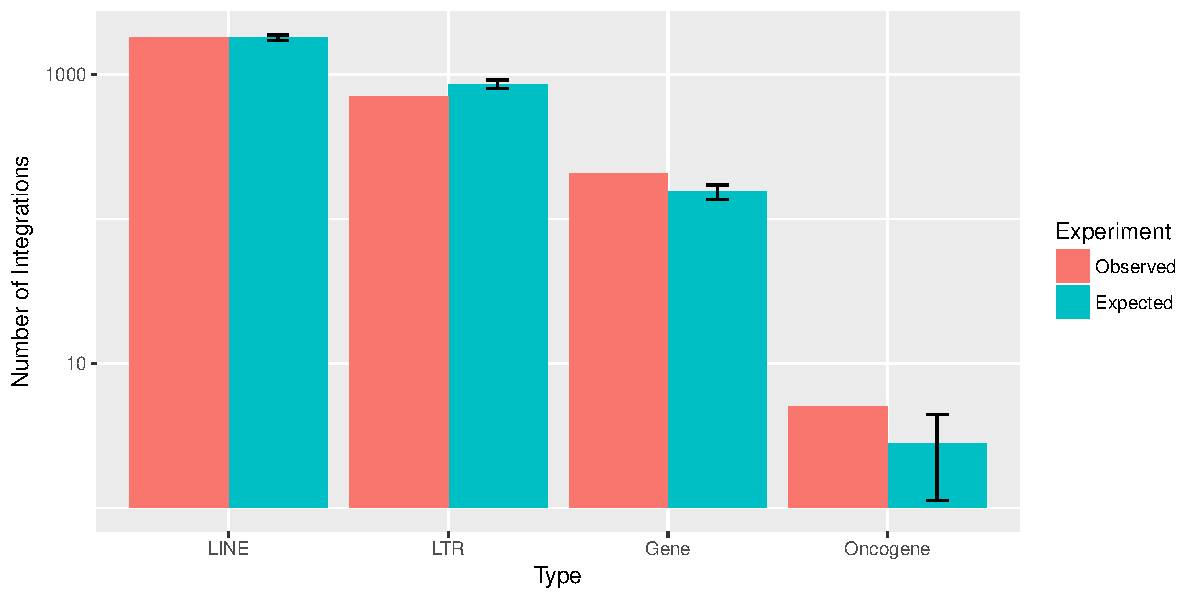
\includegraphics[width=1\linewidth]{{results/expected.counts}.pdf}\\
\caption[Annotations of integrated regions.]
{\label{integration_counts}  {\bf Annotations of integrated regions.}  We report the number of annotations within a 10kb interval of each integration.  We also report the expected integrations from 1000 simulated experiments over the same interval.  The p-values of the observed integration counts (Z-test)  are: LINE < 6e-03;	LTR < 3e-04;  Gene < 3e-04; and	Oncogenes < 0.098.}
\end{figure}

\begin{figure}[htpb]
  \centering
  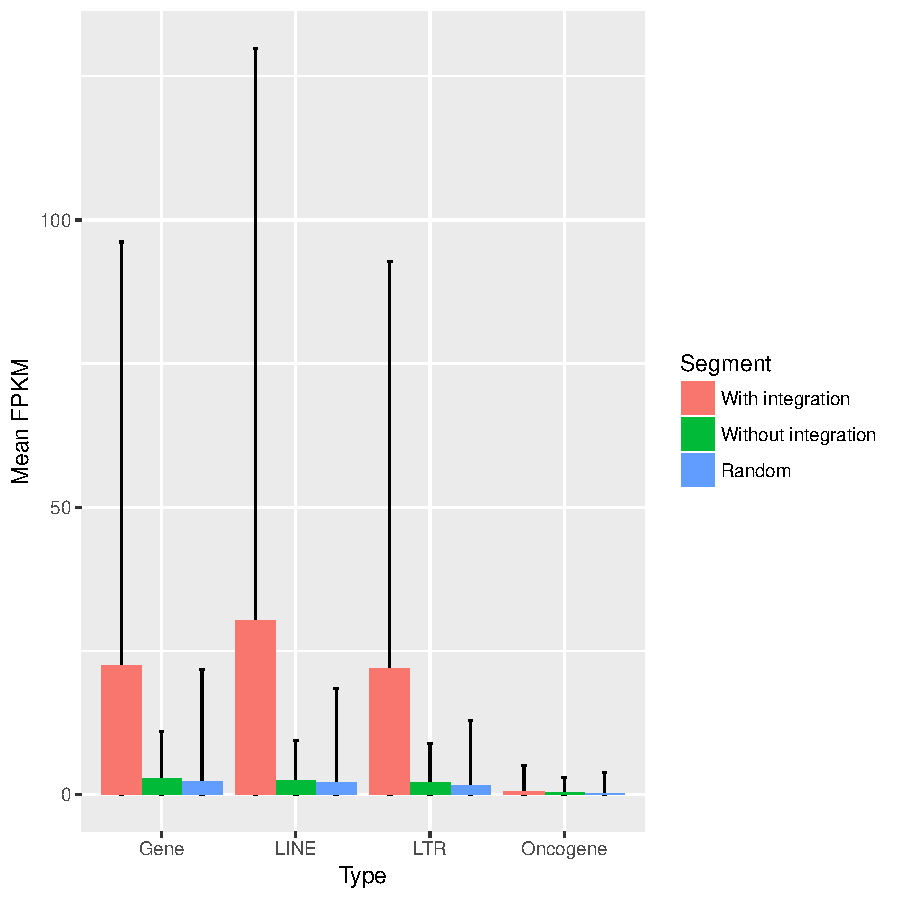
\includegraphics[width=1\linewidth]{{results/expression.summary.barplot}.pdf}\\
\caption[Expression of mRNA transcripts in genomic segments with and without integrations.]
{\label{expression_transcripts}  {\bf Expression of mRNA transcripts in genomic segments with and without integrations.}  We report the mean FPKM expression of annotated features in genomic segments with and without integrations.  For a given integration in a sample, we select a 10kb flanking region around the integration site.  We then report the expression level in samples that have an integration in this region and samples that do not.  In addition, we report the expression level randomly selected segments as a baseline. The p-values for the paired Wilcoxon signed rank test of the difference in FPKM expression for genomic segments with and mean FPKM expression in segments without integrations are: LINE < 1e-12;	LTR < 1e-10;  Gene < 1e-10; and	Oncogenes < NA.}
\end{figure}

\begin{figure}[htpb]
  \centering
  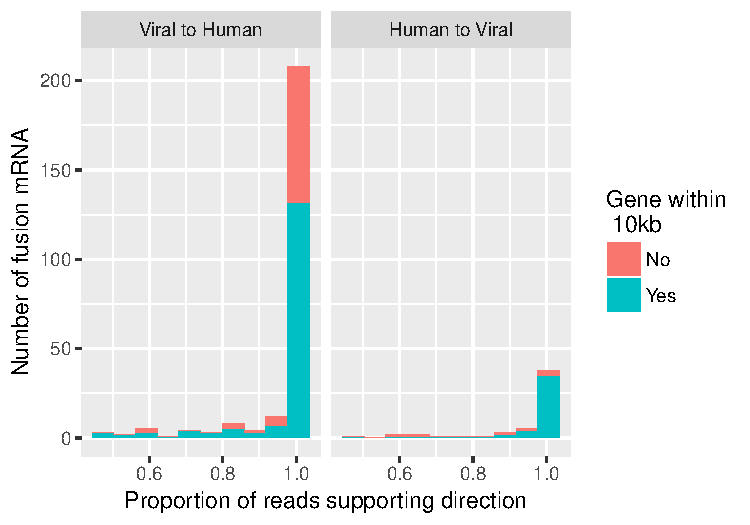
\includegraphics[width=1\linewidth]{{results/rna_direction.summary.histogram}.pdf}\\
\caption[Fusion reads supp.]
{\label{mrna_directions}  {\bf Orientation of the mRNA fusion transcripts.}  We report orientation of the fusion mRNA sequences and support for the orientation.  Orientation is inferred from the paired end reads under the assumption that the viral read is always oriented in the direction of the viral genome, and support for the orientation is computed as the proportion of paired end reads supporting that orientation.  In addition, we report whether there is a gene within 10kb of the fusion mRNA read.}
\end{figure}

\begin{figure}[htpb]
  \centering
  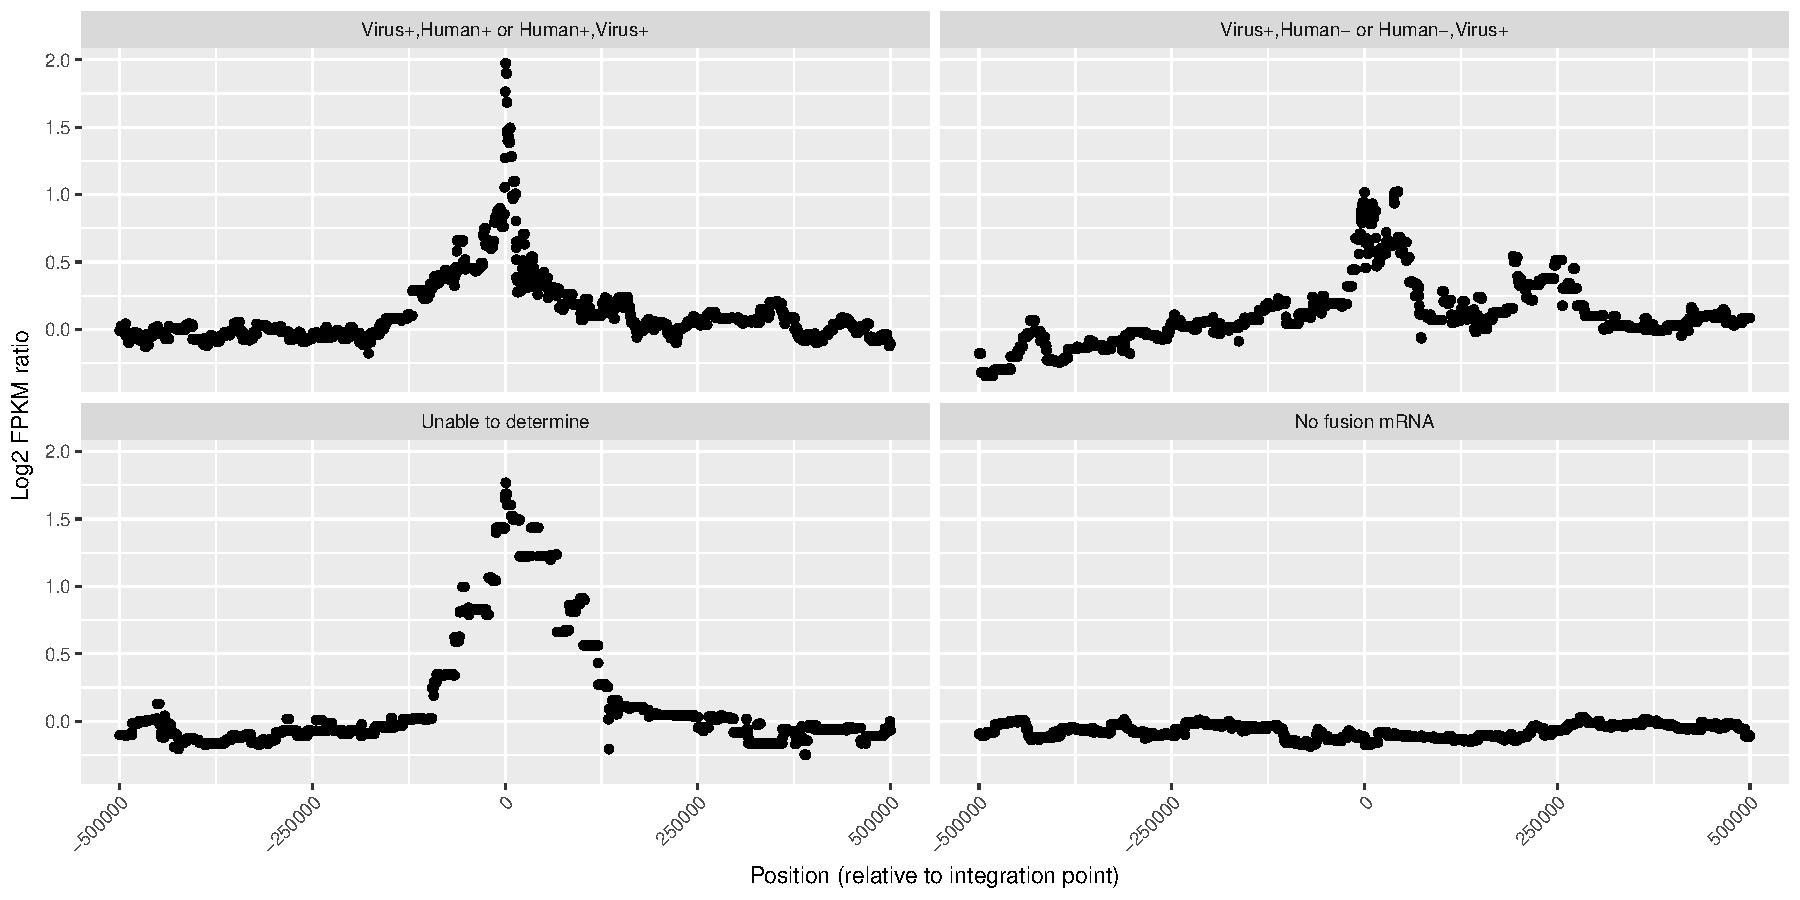
\includegraphics[width=1\linewidth]{{results/updown}.pdf}\\
\caption[Fusion reads supp.]
{\label{updown}  {\bf Average log-fold expression change around integration point.}  We report the average log-fold expression change around an integration point.  The position is reported relative to the integration point in the human genome.  We separate out the segments into four categories, based upon the orientation of the fusion mRNA reads within the genomic interval.   Orientation is determined when at least 75\% of the the paired end reads supporting a fusion mRNA have the same orientation, otherwise it is listed as unable to be determined.  Finally, some segments do not contain fusion mRNAs and are shown separately.}
\end{figure}


%\begin{table*}[htb]
%\centering
%\caption{Simulated datasets. Results on the simulated model conditions.  We report the recall and precision for each method across various model conditions.  The model conditions vary by the amount of evolution between the HPV16 strains and the reference HPV16 strain.  Easy conditions contain HPV16 strains with 99\% similarity to the reference, medium with 95\% similarity, and hard with 90\% similarity.  Methods that failed to complete are marked on the table.  VERSE failed to complete on the last step of integration detection, but we were able to recover the list of suspected integrations from the log file; we scored these results but mark them with an asterisk to denote that the values would change had VERSE been able to run to completion. }
%\label{simulation}
%\begin{tabular}{|l|r|r|r|r|r|r|}
%\hline
%Model Condition        & Total True Sites & ViralHMM      & ViralHMM\_mod  & Viraj            & VERSE            & ViralSeqFus      \\ \hline
%                       &                    & Recall/Precision  & Recall/Precision & Recall/Precision & Recall/Precision & Recall/Precision \\ \hline
%Easy HPV16 strain 13  & 987                 & 0.977/0.867   & 0.974/0.971      &  0.973/0.965               & 0.675/0.420$^*$           & 0.562/NA$^*$          \\ \hline
%Easy HPV16 strain 15  & 990                 & 0.970/0.912   &  0.977/0.988      &  Running               & Runinng           & Runinng         \\ \hline
%Easy HPV16 strain 17  & 990                 & 0.970/0.874   &  0.977/0.978      &  Running               & Runinng          & Runinng          \\ \hline
%Medium HPV16 strain 38  &     985          & 0.974/0.920    &  0.971/0.974      &  0.970/0.964         & 0.667/0.649$^*$           & 0.295/NA$^*$          \\ \hline
%%Medium HPV16 strain 75   &   985          & 0.662/0.836    &        &                  & Failed          & Running          \\ \hline
%%Medium HPV16 strain 77   &   983       & 0.623/0.808       &        &                  & Failed          & Running          \\ \hline
%Hard HPV16 strain 65 & 992                 & 0.960/0.881   &   0.961/0.978     &                  & Runinng          & Running          \\ \hline
%Hard HPV16 strain 123 & 983                 & 0.949/0.887   &   0.973/0.969     & 0.972/0.970                 & Failed          & 0.103/NA$^*$          \\ \hline
%Hard HPV16 strain 125 & 979             & 0.942/0.875       &   0.971/0.966     & 0.962/0.967                 & Failed          & 0.127/NA$^*$          \\ \hline
%
%\end{tabular}
%\end{table*}

%\subsection{RNA-seq cell line datasets}
%\begin{table*}[]
%\centering
%\caption{HCC Cell-line RNA-seq data.  RNA-seq data from four cell lines with experimentally verified fusion transcripts.}
%\label{rnaseq_hcc_cellline}
%\begin{tabular}{|l|l|l|l|l|l|}
%\hline
%Sample  & Span position (Orientation) in human genome                                                                                                 & Viral-HMM & Viraj & Virus-Finder 2 & ViralSeqFus \\ \hline
%HKCI-4  & chr4:54908780-54915241(+)                                                                                                                   & Yes       & Yes      & Yes            &        Running     \\ \hline
%        & chr5:1295559-1295834 (+)                                                                                                                    & Yes       &    Yes   & Yes            &           Running  \\ \hline
%        & chr8:41493923-41494204 (+)                                                                                                                  & Yes       &    Yes   & Yes            &           Running  \\ \hline
%        & chr13:115070262-115070459 (+)                                                                                                               & Yes       &   Yes    & Yes            &          Running   \\ \hline
%        &chr9:129733666-129733820 (+) & Yes       &   Yes    & No             &          Running   \\ \hline
%HKCI-5B & chr7:98532127-98532327 (+)                                                           & Yes       &  Yes     & Yes            &       Running    \\ \hline
%        & chr16:30408209-30408356 (+)                                                                                                                 & Yes       &   Yes    & Yes            &          Yes   \\ \hline
%HKCI-7  & chr4:99949575-99949439 (-)                                                                                                                  & Yes       &   Yes    & Yes            &          Running   \\ \hline
%        & chr11:68887645-68887577 (-)                                                                                                                 & Yes       &   Yes    & Yes            &         Running    \\ \hline
%        & chr11:14159090-14159048 (-)                                                                                                                 & No        &   No    & No             &        Running     \\ \hline
%HKCI-11 & chr4:53063790-53063967 (+)                                                                                                                  & Yes       &  Yes     & Yes            &       Running      \\ \hline
%\end{tabular}
%\end{table*}

%\subsection{HCC WGS patient results}
%Of the 22 experimentally verified integration points, Viral-HMM was able to detect 21 of the points, VERSE 8 of the points, and ...  Note that in the VERSE paper, the authors reported that they were able to detect 16 out of the 22 points.  We had difficulties in running VERSE on our samples, and tools used within the VERSE pipeline produced very large uncompressed SAM files (up to 1.2 TB in size).  We attempted to fix this by having VERSE output compressed BAM files, which allowed several of the failed runs to complete, but not all.  We suspect that with more efficient use of piping, VERSE could avoid producing many of the large files and would be able to complete on our system and potentially achieve the results reported in their paper.

%\begin{table*}[]
%\centering
%\caption{HCC WGS patient results.  Results on detection of 22 experimentally verified integration points across 13 samples taken from patients with HCC.}
%\label{my-label}
%\begin{tabular}{|l|l|l|l|l|l|}
%\hline
%Sample & Integration breakpoints in human genome & Viral-HMM & Viraj & VERSE                                & VirusSeqFus \\\hline
%145T   & chr19: 30303492                         & Y         &       & Y                                    & Running     \\\hline
%       & chr19: 30303498                         & Y         &       & Y                                    & Running     \\\hline
%177T   & chr3: 196625752                         & Y         &       & N                                    & Running     \\\hline
%180N   & chr2: 216280279                         & Y         &       & Running & Running     \\\hline
%186T   & chr19: 36214005                         & Y         &       & Y & Running     \\\hline
%       & chr19: 36214017                         & Y         &       & Y & Running     \\\hline
%198T   & chr5: 1269387                           & Y         &       & Y                                    & Running     \\\hline
%       & chr5: 1269405                           & Y         &       & Y                                    & Running     \\\hline
%26T    & chr18: 107920                           & Y         &       & Running & Running     \\\hline
%200T   & chr19: 30315003                         & Y         &       & Y & Running     \\\hline
%       & chr19: 30315365                         & Y         &       & Y & Running     \\\hline
%268T   & chr19: 30298787                         & Y         &       & Y                                    & Running     \\\hline
%       & chr5: 1292391                           & Y         &       & N                                    & Running     \\\hline
%43T    & chr3: 196625710                         & Y         &       & N                                    & Running     \\\hline
%46T    & chr5: 1295367                           & Y         &       & N                                    & Running     \\\hline
%70T    & chr19: 36212331                         & Y         &       & Running & Running     \\\hline
%       & chr19: 36212311                         & Y         &       & Running & Running     \\\hline
%71T    & chr3: 196625776                         & Y         &       & N                                    & Running     \\\hline
%       & chr19: 36213141                         & Y         &       & Y                                    & Running     \\\hline
%       & chr19: 36213136                         & Y         &       & Y                                    & Running     \\\hline
%       & chr5: 1292403                           & N         &       & N                                    & Running     \\\hline
%95T    & chr19: 36212564                         & Y         &       & Y                                    & Running    \\\hline
%\end{tabular}
%\end{table*}

%\subsection{HCC TCGA matched paired samples}
%We ran Viral-HMM on TCGA-LIHC patient samples in which there existed both WGS from tumor and normal blood samples, and RNA-seq of tumor samples.  
%
%TODO:  Graph coverage near/at integration sites, graph hotspots
%\begin{figure}[htpb]
%  \centering
%  \includegraphics[width=1\linewidth]{results/TCGA-BW-A5NP.png}\\
%\caption[Integration sites recovered from patient TCGA-BW-A5NP.]
%{\label{TCGA-BW-A5NP}  {\bf Integration sites recovered from patient TCGA-BW-A5NP.}  Blue lines represent integrations found from the WGS data.  Red lines represent integrations found from the RNA-Seq data.}
%\end{figure}
%
%\begin{figure}[htpb]
%  \centering
%  \includegraphics[width=1\linewidth]{results/TCGA-CC-5262.png}\\
%\caption[Integration sites recovered from patient TCGA-CC-5262.]
%{\label{TCGA-CC-5262}  {\bf Integration sites recovered from patient TCGA-CC-5262.}  Blue lines represent integrations found from the WGS data.  Red lines represent integrations found from the RNA-Seq data.}
%\end{figure}
%
%\begin{figure}[htpb]
%  \centering
%  \includegraphics[width=1\linewidth]{results/TCGA-CC-A1HT.png}\\
%\caption[Integration sites recovered from patient TCGA-CC-A1HT.]
%{\label{TCGA-CC-A1HT}  {\bf Integration sites recovered from patient TCGA-CC-A1HT.}  Blue lines represent integrations found from the WGS data.  Red lines represent integrations found from the RNA-Seq data.}
%\end{figure}


\section{Discussion}

\section{Conclusion}

\section*{Acknowledgements}
The results published here are in whole or part based upon data generated by the TCGA Research Network: \href{http://cancergenome.nih.gov/}.

%\section{Notes}
%
%Need to focus on flanking regions of 25kb in paper.
%
%
%[1] M. Kadaja, A. Sumerina, T. Verst, M. Ojarand, E. Ustav, and M. Ustav, “Genomic instability of the host cell induced by the human papillomavirus replication machinery.,” EMBO J., vol. 26, no. 8, pp. 2180–91, 2007.
%
%E1 protein is replicon origin recognition factor and viral helicase, which with E2, helps recruit(?) host cell replication complexes onto the HPV origin.  High E1 result in high recruitment of host replication complex at virus origin site.
%
%Flanking DNA can be amplified, up to 12kb, with total amplicon size 25kb.  The amplification locus could be a target for genomic re-arrangments due to recruitment of DDR mechanisms.  In addition, onion-skin model of replication cuz breaks, fragments

%[1] M. Kadaja, H. Isok-Paas, T. Laos, E. Ustav, and M. Ustav, “Mechanism of genomic instability in cells infected with the high-risk human papillomaviruses,” PLoS Pathog., vol. 5, no. 4, 2009.
%
%
%
%[1] Z. Jiang, S. Jhunjhunwala, J. Liu, P. M. Haverty, M. I. Kennemer, Y. Guan, W. Lee, P. Carnevali, J. Stinson, S. Johnson, J. Diao, S. Yeung, A. Jubb, W. Ye, T. D. Wu, S. B. Kapadia, F. J. De Sauvage, R. C. Gentleman, H. M. Stern, S. Seshagiri, K. P. Pant, Z. Modrusan, D. G. Ballinger, and Z. Zhang, “The effects of hepatitis B virus integration into the genomes of hepatocellular carcinoma patients The effects of hepatitis B virus integration into the genomes of hepatocellular carcinoma patients,” pp. 593–601, 2012.

%Runthrough for HBV, directional, need to make a clear graph
%\section{Cell lines}
%HPV16-positive W12 cell line both viral and integrated HPV genomes in early stages, lost of plasmids in later stages

\section*{Funding}

\section*{Disclosures}
VB is a partner in Digital Proteomics, LLC (DP), which licenses and sells computational tools for analyzing mass spectrometry data. The terms of this arrangement have been reviewed and approved by the University of California, San Diego in accordance with its conflict of interest policies. DP was not involved in the research presented here
%\bibliographystyle{natbib}
%\bibliographystyle{achemnat}
%\bibliographystyle{plainnat}
%\bibliographystyle{abbrv}
%\bibliographystyle{bioinformatics}
%
%\bibliographystyle{plain}
%
%\bibliography{Document}

\bibliographystyle{natbib}
\bibliography{main}
\end{document}




